\section{Installation}

\begin{frame}{}
    \tableofcontents[currentsection]
\end{frame}


\begin{frame}{Installation}
    % try it on my own on a second computer
    % try also what happens with Python 3.12 or 3.13
    The three requisites are:
    \begin{enumerate}
        \item Python 3.10 or 3.11.
        \item VSCode.
        \item GridCal wheels.
    \end{enumerate}
\end{frame}

\begin{frame}{Python installation}
    \begin{itemize}
        \item For instance, download Python 3.10.9 from \href{https://www.python.org/downloads/release/python-3109/}{https://www.python.org/downloads/release/python-3109/}.
        \item Make sure to add Python to the PATH.
    \end{itemize}
    \begin{figure}[!htb]
        \centering
        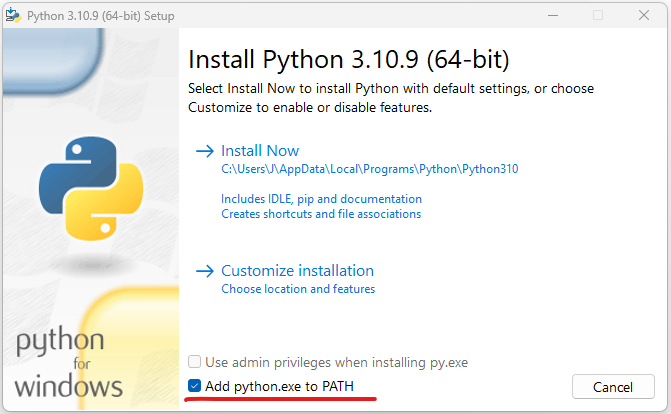
\includegraphics[width=0.6\textwidth]{Images/python_install.png}
        \caption{Python installation.}
        \label{fig:python_installation}
    \end{figure}
\end{frame}

\begin{frame}{VSCode installation}
    \begin{itemize}
        \item Download VSCode from \href{https://code.visualstudio.com/}{https://code.visualstudio.com/}.
        \item Install the Python extension.
    \end{itemize}
        \begin{figure}[!htb]
        \centering
        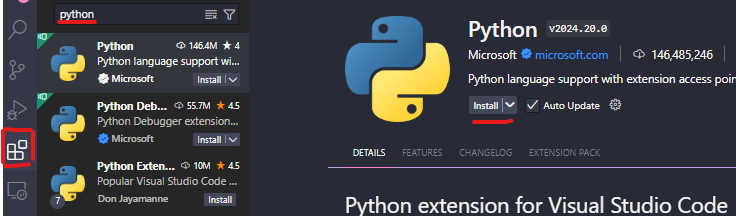
\includegraphics[width=0.6\textwidth]{Images/python_vscode.png}
        \caption{Python VSCode extension.}
        \label{fig:vscode_installation}
    \end{figure}
\end{frame}

\begin{frame}{GridCal installation}
    \begin{itemize}
        \item Create a virtual environment in VSCode: Ctrl+Shift+P,  then Python: Create Environment.
        \item Activate with \fbox{"./.venv/Scripts/Activate"}.
        \item Install the latest alpha GridCal release: \fbox{pip install GridCal==5.3.0a1}.
        \item Verify the installation with \fbox{pip list}.
    \end{itemize}
    Open the interface:
    \begin{itemize}
        \item Windows: 
        \begin{center}
            % \fbox{python -c "from GridCal.ExecuteGridCal import run; run()"}
            \fbox{python -c "from GridCal.ExecuteGridCal import runGridCal; runGridCal()"}
        \end{center}
        \item Unix: 
        \begin{center}
            \fbox{python3 -c "from GridCal.ExecuteGridCal import runGridCal; runGridCal()"}
            % \fbox{python3 -c "from GridCal.ExecuteGridCal import run; run()"}
        \end{center}
    \end{itemize}
    % CTRL+SHIFT+P, create virtual env
    % .\.venv\Scripts\Activate
    % pip install GridCal==5.3.0a1
    % https://stackoverflow.com/questions/54776324/powershell-bug-execution-of-scripts-is-disabled-on-this-system
\end{frame}
